\documentclass[11pt]{article}
\usepackage[margin=1in]{geometry}
\usepackage{booktabs}
\usepackage{graphicx}
\usepackage{float}
\begin{document}
\section*{Supplementary Step 4 Visualization Report}
\subsection*{Overview}
\begin{tabular}{p{0.36\linewidth}p{0.54\linewidth}}
\toprule
Metric & Value\\
\midrule
Representative geometry session & PID001 / 2025-11-06\_008\\
Included participant-sessions from Step 4 & 36\\
Abstract onset-locked epochs used & 539\\
Concrete onset-locked epochs used & 536\\
Trials dropped for fixed epoch window & 0\\
Epoch window & -3.5 s to 13.2 s around question onset\\
Baseline & -2.0 s to 0.0 s\\
Single-time comparison & 9.0 s\\
\bottomrule
\end{tabular}
\paragraph{Rendering note.} The original example requested a brain-surface sensor rendering. In this environment, the report uses the participant digitization point cloud together with source, detector, channel, and pair geometry because the local \texttt{pyvista}/\texttt{fsaverage} rendering stack is not available.
\subsection*{Representative Sensor Geometry}
\begin{figure}[H]
\centering
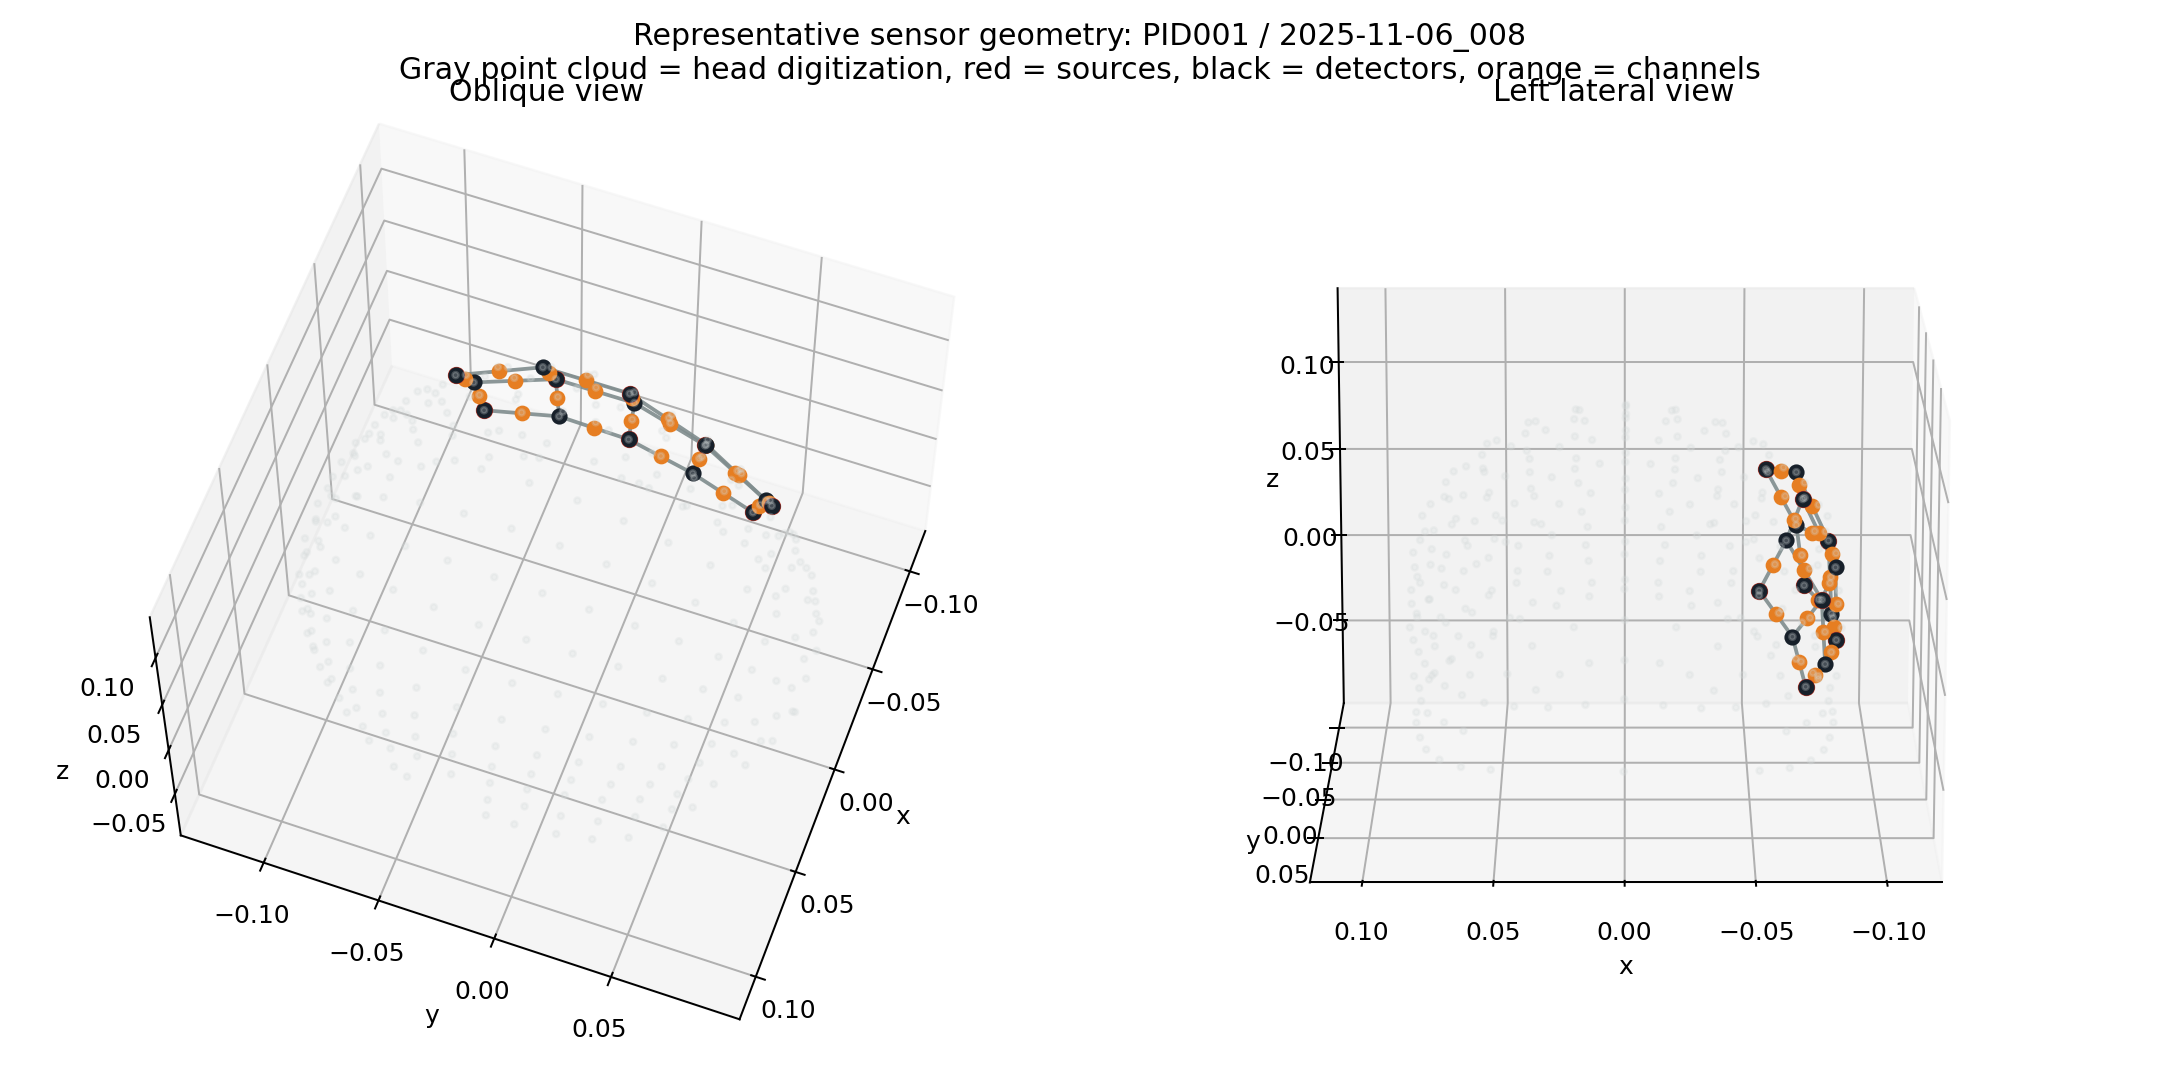
\includegraphics[width=0.95\linewidth]{../../figures/step4_visualization/representative_sensor_geometry.png}
\caption{Representative optode, channel, and source-detector-pair geometry for one included participant-session. Short pairs are shown with dashed orange lines.}
\end{figure}
\subsection*{Condition-Specific Topography Over Time}
\begin{figure}[H]
\centering
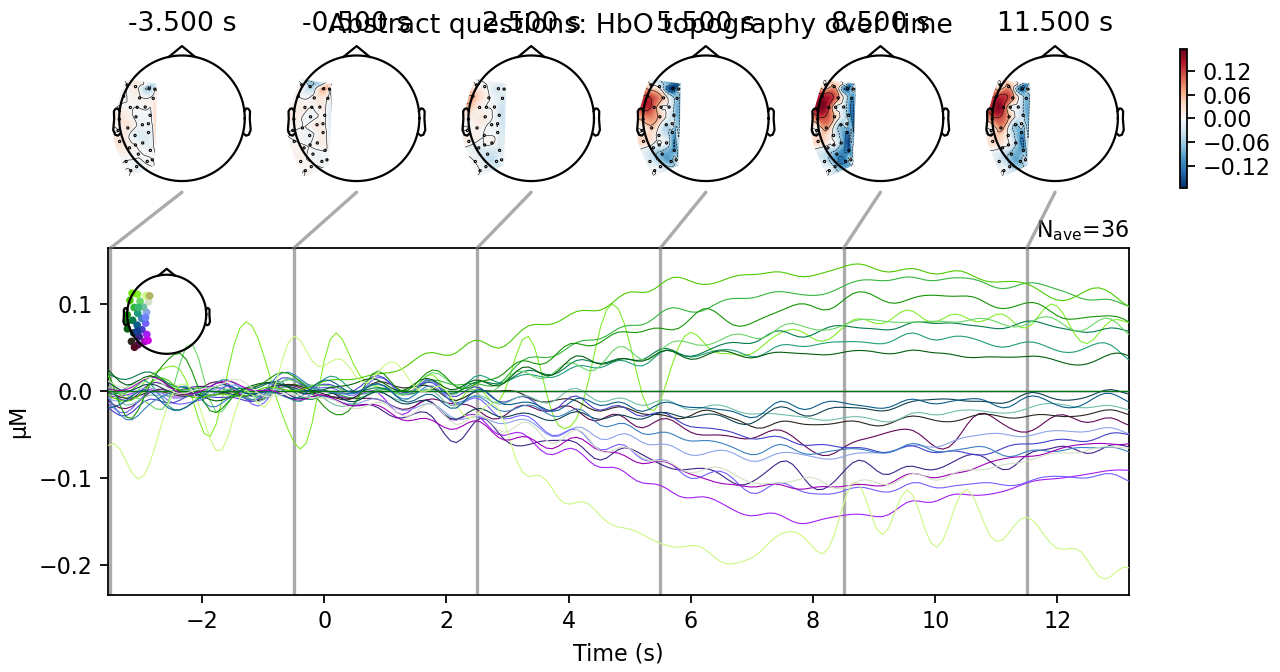
\includegraphics[width=0.95\linewidth]{../../figures/step4_visualization/abstract_hbo_joint.png}
\caption{Grand-average HbO topography over time for abstract questions, aligned to question onset.}
\end{figure}
\begin{figure}[H]
\centering
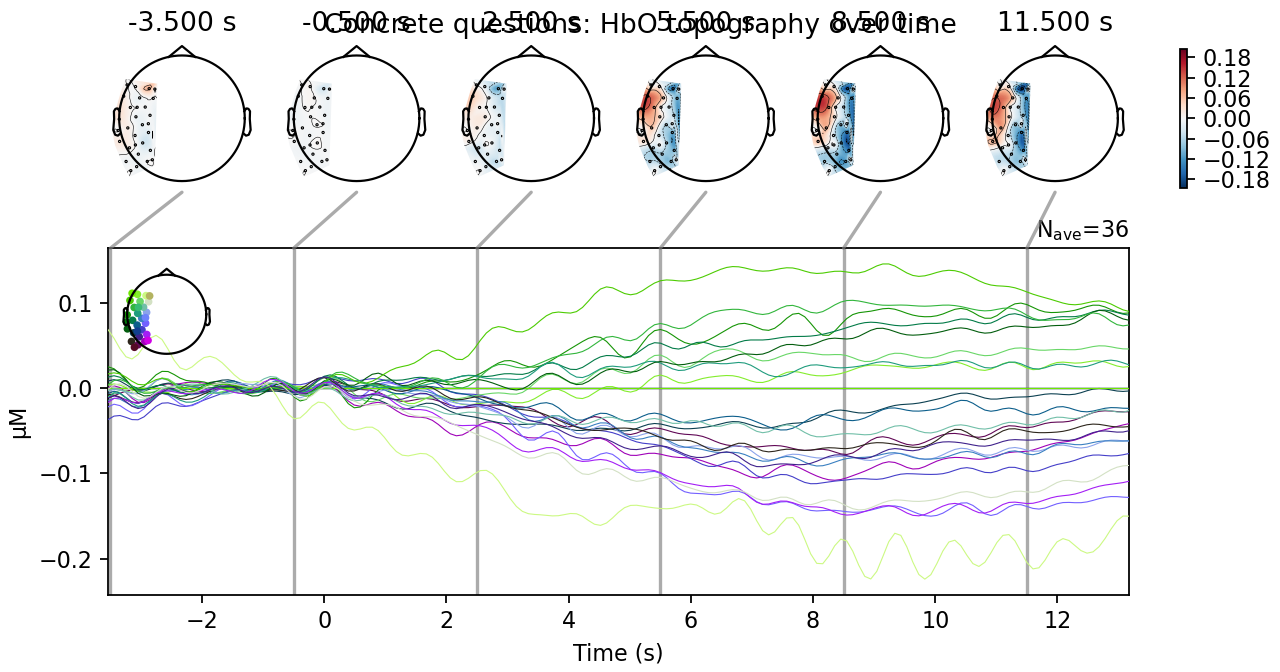
\includegraphics[width=0.95\linewidth]{../../figures/step4_visualization/concrete_hbo_joint.png}
\caption{Grand-average HbO topography over time for concrete questions, aligned to question onset.}
\end{figure}
\subsection*{Single-Time-Point Condition Comparison}
\begin{figure}[H]
\centering
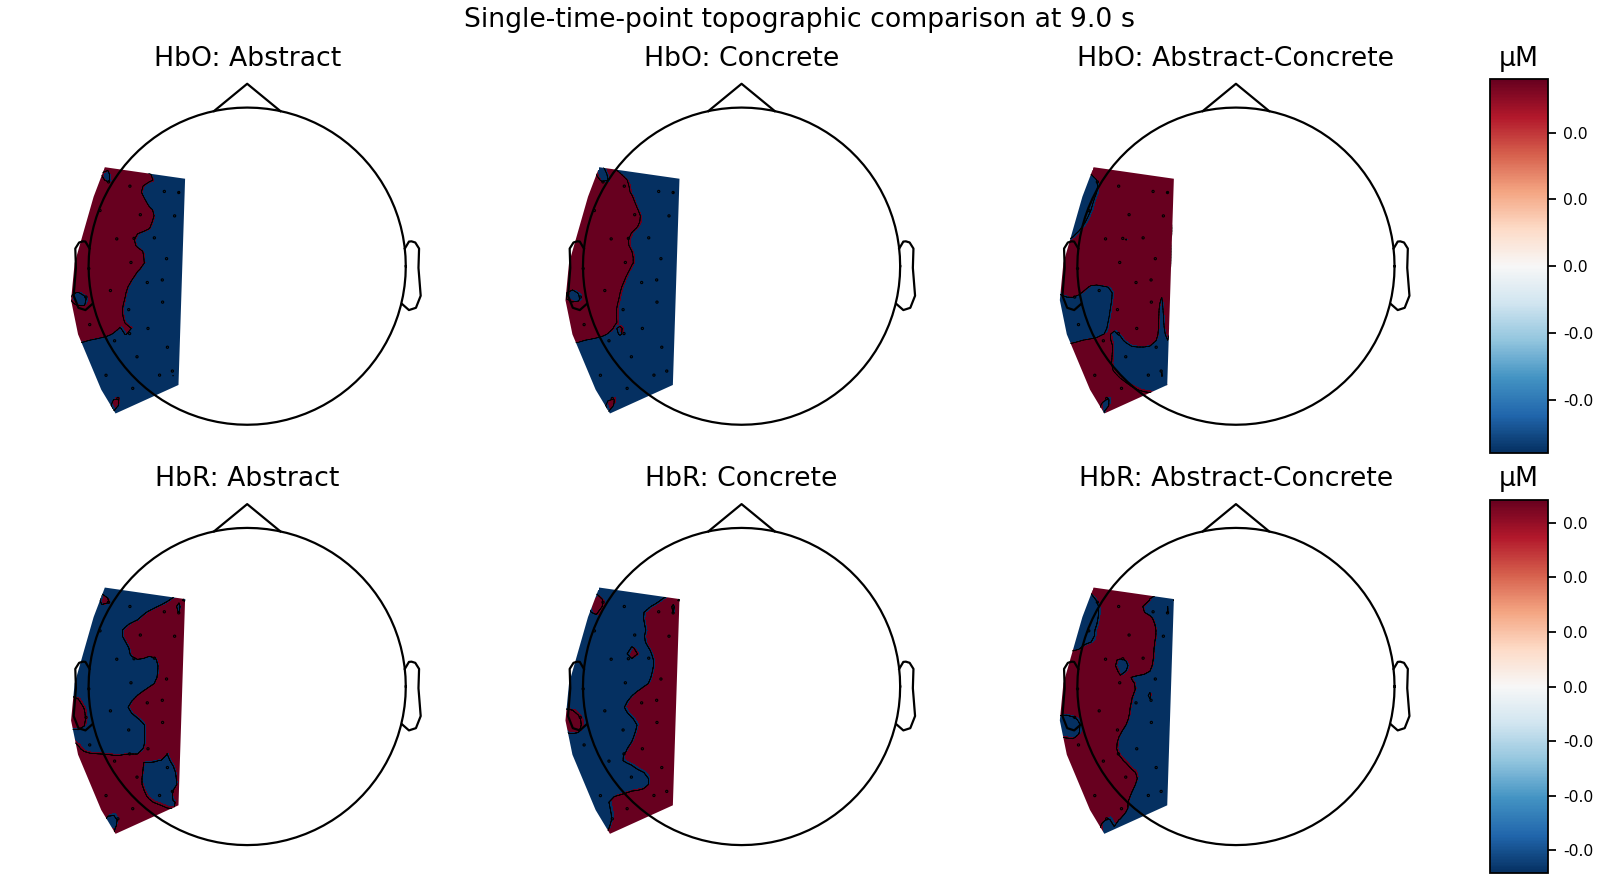
\includegraphics[width=0.95\linewidth]{../../figures/step4_visualization/abstract_concrete_single_time_comparison.png}
\caption{Condition comparison at one time point for HbO and HbR, with the abstract-minus-concrete difference shown in the rightmost column.}
\end{figure}
\end{document}
